\section{Semantički upoređivač}
\label{sec:ImplementationComparer}

Implementacija algoritma upoređivača opisana u poglavlju \ref{chp:ASTComparing} se svodi na implementaciju funkcija za poređenje za svaki tip AST čvora. Te funkcije su enkapsulirane u klase koje implementiraju interfejs za upoređivač čvorova. Te klase nisu javne, tako da se poređenje vrši kroz upoređivač koji poredi instance tipa \texttt{ASTNode}, a koji putem refleksije određuje konkretni tip čvorova i, ukoliko su tipovi isti, pronalazi konkretni upoređivač i poziva operaciju interfejsa upoređivača. Upoređivači međusobno pozivaju jedni druge, kako bi se logika poređenja uprostila --- pošto se naredbe deklaracije sastoje od specifikatora deklaracije i liste deklaratora, upoređivač naredbi deklaracije može pozivati upoređivač za specifikatore deklaracije i upoređivač za listu deklaratora. 

Upoređivač kao rezultat svog rada vraća kolekciju potencijalnih problema (upozorenja ili grešaka) koje je detektovao prilikom analize. Ovakav pristup je odabran zbog lakoće testiranja upoređivača, s obzirom da se može očekivati određena kolekcija problema za određeni izvorni k\^od. Problem se modeluje kao apstraktna klasa \texttt{BaseIssue} dok se upozorenja ili greške modeluju kroz njene konkretizacije \texttt{BaseWarning} i \texttt{BaseError}. Konkretne greške, kao što su npr. nedostatak deklaracija se mogu onda modelovati kao konkretizacije ovih klasa u zavisnosti od ozbiljnosti problema. Primer izlaza upoređivača za algoritam \emph{swap} se može videti na slici \ref{fig:ComparerSwap}.

\begin{figure}[h!]
\centering
%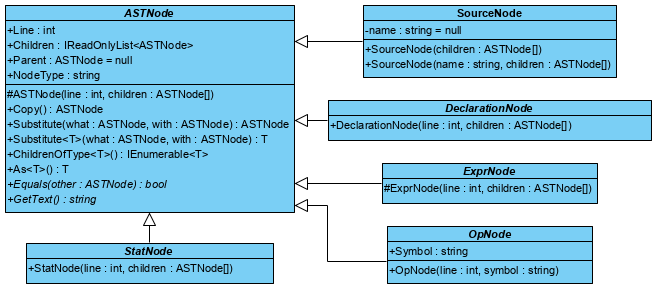
\includegraphics[scale=0.7]{images/uml/ASTNode.png}
\caption{Rezultat rada upoređivača za \texttt{swap} algoritam.}
\label{fig:ComparerSwap}
\end{figure}
